\section{Signaling insulation between BMP and \tgf}
\label{insulation:bmpTgfb}


 
  \begin{figure}[!bt]
  \centering
  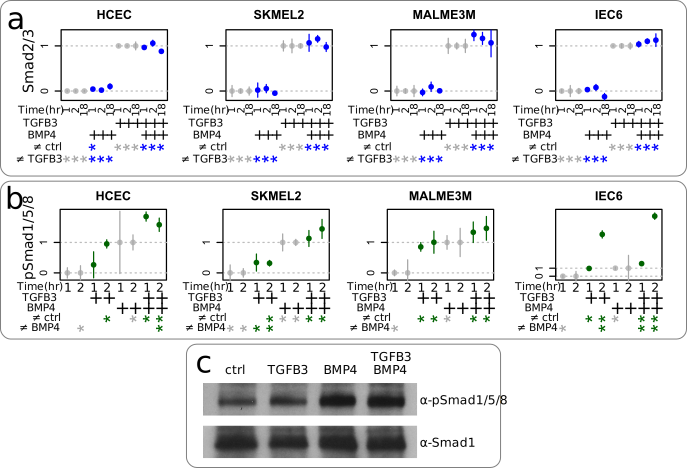
\includegraphics[width=6.5in]{FIGS/insulation/bmpTgfbInsulation.pdf}
  {\singlespacing 
  \caption[BMP4 and \tgf\ do not compete for Smad4 (all data).]
        { The \tgf\ and BMP signaling pathways are additive,
          and do not compete for Smad4. \b{a}, BMP4 causes no
          modulation of Smad2/3 responses at
          both short (1-2hr) and long (18hr) timepoints across all
          cell lines tested. \b{b}, \tgf 3 additively modulates pSmad1/5/8
          responses to BMP4. \b{c}, Measurement of \tgf 3/BMP4 crosstalk by
          Western is consistent with the imaging data. SKMEL2, 2hr treatment.
          \b{a,b}, Y-axes, normalization, and
          p-values as in \ar{fig:insulation:wntTgfbInsulation}. 
          Concentrations (1 and 2hr): 0.2ng/mL \tgf 3, 5ng/mL BMP4. Concentrations (18hr): 10ng/mL \tgf 3, 25ng/mL BMP4.
          Western courtesy Curtis A. Thorne (Altschuler \& Wu lab, UT
          Southwestern).
          }
  \label{fig:insulation:bmpTgfbInsulation}}
  \end{figure}



The above result is perhaps not so surprising,
that two pathways (Wnt3A and \tgf 3) lacking any shared core components do
not modulate one another during signal transduction. 
Under this rationale the BMP2/4 and \tgf 1/3 pathways
might then be expected to interact, given their shared requirement
for Smad4. Indeed, the claim of intra-\tgfbsf\ crosstalk 
via Smad4 competition has been cited in many reviews and papers,
but to my knowledge has not been directly tested
(\ar{pathways:tgfb:crosstalk}). I therefore
decided to use the same experimental setup as above to measure
the extent of crosstalk between BMP4 and \tgf 3
(\ar{fig:insulation:bmpTgfbInsulation}). The essential data is
again summarized in a simpler figure
(\ar{fig:insulation:bmpTgfbSummary}). If these pathways do 
compete for Smad4, then co-treatment with saturating concentrations
of both ligands (to maximize sequestration of Smad4) should cause one or
both pathways to be attenuated.

  \begin{figure}[!bt]
  \centering
  \includegraphics[width=5in]{FIGS/insulation/bmpTgfb_summary.pdf}
  {\singlespacing 
  \caption[BMP4 and \tgf\ do not compete for Smad4 (summary).]
        { Summary figure showing the lack of Smad4 competition between BMP4 and \tgf 3,
          limited to SKMEL2s and HCECs at 2hrs.
          \b{a}, There is additive signaling crosstalk from \tgf 3 to
          pSmad1/5/8, but not from BMP4 to Smad2/3.
          \b{b}, At the same time, the transcriptional output from the combined
          pathways also appears to be additive.
          \b{c}, Smad4 RNAi reduces protein levels of Smad4 in HCECs.
          Histone H3B serves as a loading control. 
          \b{d}, Smad4 RNAi in HCECs reduces overall \tgf 3 responsiveness (top)
          but not pSmad1/5/8 responsiveness (middle), while the signaling
          crosstalk between \tgf 3 and BMP4 remains approximately
          additive. Thus, competition for Smad4 does not cause cross-pathway
          signaling inhibition between \tgf 3 and BMP4. Normalization
          for \b{d} uses the control and single-ligand responses from
          the scramble siRNA treatment to define 0 and 1.
          Y-axes, normalization, and
          p-values as in \ar{fig:insulation:wntTgfbInsulation}. Daggers
          indicate significant departure from pathway insulation.
          Data for \b{a} from \ar{fig:insulation:bmpTgfbInsulation}.
          Data for \b{b} from \ar{fig:insulation:expressionXtalk}.
          Western courtesy Curtis A. Thorne (Altschuler \& Wu lab, UT
          Southwestern).
          }
  \label{fig:insulation:bmpTgfbSummary}}
  \end{figure}
    
  
  
BMP4 treatment
had absolutely no effect on Smad2/3 in any cell line
(\ar{fig:insulation:bmpTgfbInsulation}a;
 \ar{fig:insulation:bmpTgfbSummary}a,top). There is crosstalk
in the other direction:
treatment by \tgf 3 is sufficient to activate pSmad1/5/8, and
the presence of both ligands yields an additive behavior
(\ar{fig:insulation:bmpTgfbInsulation}b). Importantly, these
two pathways also have an approximately-additive effect on
transcription of their shared downstream target, Smad7
(\ar{fig:insulation:expressionXtalk}; \ar{fig:insulation:bmpTgfbSummary}b,top).
As noted
in \ar{pathways:tgfb:smads}, while the BMP2/4 and \tgf\ pathways
are generally considered to be distinct, they have been shown to
cross-activate one another in various settings.
Western blotting was not quantitative enough to confirm the
activation of pSmad1/5/8 by \tgf 3, but is consistent with an
absence of negative cross-regulation
(\ar{fig:insulation:bmpTgfbInsulation}c). In any case,
both the insulation of Smad2/3 from BMP4 and the additive
crosstalk between \tgf 3 and pSmad1/5/8 directly argue against
competitive inhibition between these pathways
during signal transduction.


I then wondered if the absence of inhibitory crosstalk
between BMP4 and \tgf 3 was a context-dependent phenomenon.
For example, the additive behavior is consistent
with the quantity of Smad4 being so high
as to be non-limiting, in which case both pathways would effectively have
distinct pools of Smad4 (as in \ar{fig:insulation:crosstalk}c).
I therefore used siRNA to knock down Smad4 in order to make Smad4 a
limiting factor in an effort to modulate the form of crosstalk
(e.g. to a non-additive form as in \ar{fig:insulation:crosstalk}d).


As a consequence of Smad4 depletion
(\ar{fig:insulation:bmpTgfbSummary}c), \tgf 3 signaling was strongly reduced overall
but was still not inhibited by co-treatment with BMP4
(\ar{fig:insulation:bmpTgfbSummary}d, top). Levels of pSmad1/5/8,
on the other hand, were not affected overall by Smad4 knockdown
(\ar{fig:insulation:crosstalk}d, top) and the effect of co-treatment
remained roughly additive. Therefore, in contrast to expectations,
BMP4 and \tgf 3 do not negatively regulate one another at all
at the level of signal transduction, and do
not compete for Smad4.

